\documentclass[aspectratio=43]{beamer}
% Theme works only with a 4:3 aspect ratio
\usetheme{CSCS}

\usepackage{tikz}

\usepackage{pgfplots}
\usepackage{pgfplotstable}
\usetikzlibrary{pgfplots.groupplots,spy,patterns}
\usetikzlibrary{arrows.meta}
\usetikzlibrary{positioning}
\usepackage{listings}
\usepackage{color}
\usepackage{tcolorbox}
\usepackage{anyfontsize}
\usepackage{xspace}
\usepackage{graphicx}
\usepackage{pifont}

% define footer text
\newcommand{\footlinetext}{Alps User Environments}

% Select the image for the title page
\newcommand{\picturetitle}{slide-images/image5.pdf}

% fonts for maths
\usefonttheme{professionalfonts}
%\usefonttheme{serif}

\input{listing-spec.tex}

% source code listing
\newcommand\TS{\rule{0pt}{2.6ex}}       % Top strut
\newcommand\BS{\rule[-1.2ex]{0pt}{0pt}} % Bottom strut
\newcommand{\hl}[1]{\textbf{\textcolor{blue}{#1}}} % for hilighting optimal entries in tables
\newcommand{\rl}[1]{\textbf{\textcolor{red}{#1}}} % for hilighting sub-optimal entries in tables
\newcommand{\img}[1]{{\Large \textbf{IMAGE {#1}}}}
\newcommand{\hilight}[1]{\textcolor{blue!20!orange}{#1}}
\newcommand{\alps}[0]{Alps\xspace}
\newcommand{\stackinator}[0]{Stackinator\xspace}
\newcommand{\stackboxwidth}[0]{5cm}
\newcommand{\stackboxheight}[0]{1cm}
\newcommand{\stacksystemcolor}[0]{blue!10}
\newcommand{\stackbootstrapcolor}[0]{green!10}
\newcommand{\stackcolor}[0]{orange!10}

% set indent to a more reasonable level (so that itemize can be used in columns)
\setlength{\leftmargini}{20pt}

\DeclareTextFontCommand{\emph}{\color{blue!85!black}}

\author{
    \textbf{B.~Cumming},
    J.~Coles,
    T-I.~Manitaras,
    J-G.~Piccinali,
    S.~Pintarelli,
    H.~Stoppels}
\title{\centering Deploying Alternative User Environments on Alps}
\subtitle{CUG23 -- Helsinki}

\begin{document}

\setlength\labelsep   {\dimexpr\labelsep - 0.2em\relax}
\setlength\leftmargini{\dimexpr\leftmargini - 1.0em\relax}

% TITLE SLIDE
\cscstitle

\cscschapter{Setting the scene: motivation}

%-------------------------------------------
\begin{frame}[fragile]{Alps}
    Alps is the new Cray EX-based system at CSCS.

    \vspace{20pt}

    Borrow slide from Maxime's presentation showing the different vClusters

    \vspace{20pt}

    Consolidate disparate clusters onto a single Cray EX system

    \vspace{20pt}

    using CSM underneath -- each vCluster is depoloyed with its own software environment, scheduler, storage and network isolation

\end{frame}
%-------------------------------------------

%-------------------------------------------
\begin{frame}[fragile]{Monolithic Software Stacks}
    \begin{columns}[T]
        \begin{column}{0.5\textwidth}
            \includegraphics[width=\textwidth]{images/stack-old.png}
        \end{column}
        \begin{column}{0.5\textwidth}

            \small

            Sites build software for users using compilers and libraries from CPE
            % point out presentations past and present
            \begin{itemize}
                \item install all the software for all the users on a shared file system.
                \item modules alongside CPE modules
            \end{itemize}

            Is CPE a solid foundation when:
            \begin{itemize}
                \item it changes every 3 months
                \item it exposes a large surface area
                \item bugs will take 3-6 months minimum for fixes to be available
            \end{itemize}
        \end{column}
    \end{columns}
\end{frame}
%-------------------------------------------

%-------------------------------------------
\begin{frame}[fragile]{Bespoke SW stacks}
    \begin{columns}[T]
        \begin{column}{0.5\textwidth}

            Build use case and workflow specific software stacks:
            \begin{itemize}
                \item only packages that are needed
                \item deployed independently of one-another
                \item deployed independently of one-another
            \end{itemize}

            Build them on a simple foundation:
            \begin{itemize}
                \item CrayOS + libfabric + Slurm + xpmemm
                \item \emph{no CPE}
                \item infrequent changes
                \item small surface area
            \end{itemize}


        \end{column}
        \begin{column}{0.5\textwidth}
            \includegraphics[width=\textwidth]{images/stack-new.png}
        \end{column}
    \end{columns}
\end{frame}
%-------------------------------------------

%-------------------------------------------
\begin{frame}[fragile]{Objectives}
    Software environments have the following objectives that make them DevOps compatible:
    \begin{itemize}
        \item reproducable from simple recipes
        \item versionable with git
        \item support easy roll back
        \item adapt to changes in the underlying system without modifying the recipe
        \item testable
    \end{itemize}
\end{frame}
%-------------------------------------------

\cscschapter{The stackinator: building environments}

%-------------------------------------------
\begin{frame}[fragile]{Stackinator}
    A tool ``stackinator'' is used to configure the software stack on the target system:

            \begin{lstlisting}[style=talkbash]
            stack-config --recipe $recipe_path \
             --system $CLUSTERNAME \
             --build /dev/shm/build
            \end{lstlisting}

    \begin{itemize}
        \item \emph{recipe}: YAML files that describe compilers, software packages, and tests for software stack
        \item \emph{system}: System config for few libraries (gcc, libfabric, xpmem, slurm, rdma-core)
        \item \emph{mount}: The installation path of the be installed (in the recipe)
        \item \emph{build}: Where the build will be performed.
    \end{itemize}

    \url{https://github.com/eth-cscs/stackinator}
\end{frame}

%-------------------------------------------
\begin{frame}[fragile]{System Configurations}
    A Spack configuration for the target vCluster that describes the handful of system dependencies.

    \begin{columns}[T]
        \begin{column}{0.5\textwidth}
        \begin{codecolumn}{packages.yaml}
            \begin{lstlisting}[style=talkyaml]
packages:
 libfabric:
  buildable: false
  externals:
  - spec: libfabric@1.15.2.0
    prefix: /opt/cray/libfabric/1.15.2.0/
 slurm:
  buildable: false
  externals:
  - spec: slurm@22-5-2
    prefix: /usr
 xpmem: ...
 rdma-core: ...
            \end{lstlisting}
        \end{codecolumn}
        \end{column}
        \begin{column}{0.5\textwidth}
        \begin{codecolumn}{compilers.yaml}
            \begin{lstlisting}[style=talkyaml]
compilers:
- compiler:
 spec: gcc@7.5.0
  paths:
   cc: /usr/bin/gcc
   cxx: /usr/bin/g++
   f77: /usr/bin/gfortran
   fc: /usr/bin/gfortran
  flags: {}
  operating_system: sles15
  target: x86_64
            \end{lstlisting}
        \end{codecolumn}
        \end{column}
    \end{columns}
\end{frame}

%-------------------------------------------
\begin{frame}[fragile]{Recipe: general configuration}

Name, mount point, default system (deprecate), the version of Spack to use and mirror configuration.

\begin{code}{\lstinline{config.yaml}}
\lstinputlisting[style=talkyaml]{src/nv-recipe/config.yaml}
\end{code}

\end{frame}
%-------------------------------------------

%-------------------------------------------
\begin{frame}[fragile]{Recipe: compiler toolchains}

todo

\begin{code}{\lstinline{compilers.yaml}}
\lstinputlisting[style=talkyaml]{src/nv-recipe/compilers.yaml}
\end{code}

\end{frame}
%-------------------------------------------

%-------------------------------------------
\begin{frame}[fragile]{Recipe: environments}

    \begin{columns}[T]
        \begin{column}{0.5\textwidth}
        \begin{codecolumn}{environments.yaml}
\lstinputlisting[style=talkyaml, firstline=1, lastline=16]{src/nv-recipe/environments.yaml}
        \end{codecolumn}
        \end{column}
        \begin{column}{0.5\textwidth}
        \begin{codecolumnnotitle}{}
\lstinputlisting[style=talkyaml, firstline=17]{src/nv-recipe/environments.yaml}
        \end{codecolumnnotitle}
        \end{column}
    \end{columns}

\end{frame}
%-------------------------------------------

%-------------------------------------------
\begin{frame}[fragile]{Stacks}
    A ``Spack Stack'' is built in layers on top of a handful of external system dependencies.
    \begin{center}
        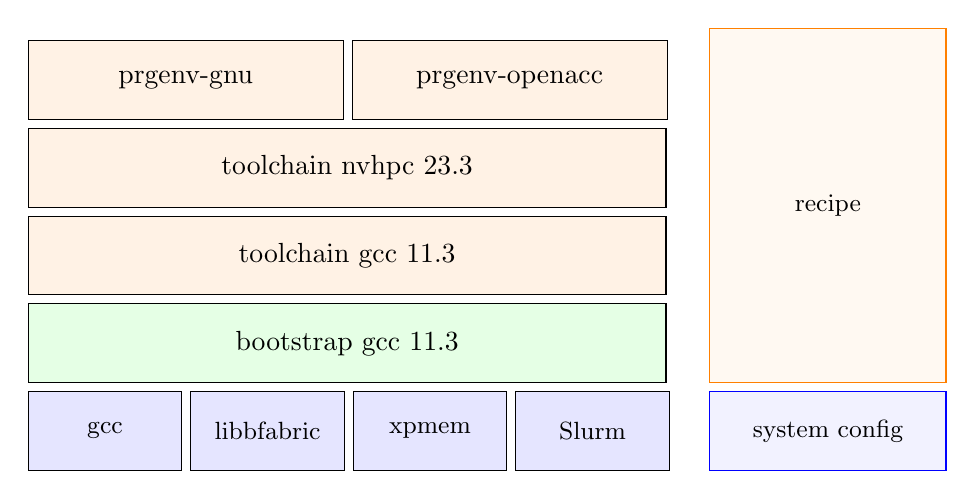
\begin{tikzpicture}
    \node[rectangle, draw=black, fill=\stacksystemcolor, minimum width=1.95cm, minimum height=1cm]
        (system_gcc) {\small gcc};
    \node[rectangle, draw=black, fill=\stacksystemcolor, minimum width=1.95cm, minimum height=1cm,
        right=0.1cm of system_gcc]
        (libfabric) {\small libbfabric};
    \node[rectangle, draw=black, fill=\stacksystemcolor, minimum width=1.95cm, minimum height=1cm,
        right=0.1cm of libfabric]
        (xpmem) {\small xpmem};
    \node[rectangle, draw=black, fill=\stacksystemcolor, minimum width=1.95cm, minimum height=1cm,
        right=0.1cm of xpmem]
        (slurm) {\small Slurm};
    \node[rectangle, draw=blue, fill=blue!5, minimum width=3cm, minimum height=1cm,
        right=0.5cm of slurm]
        (sysconfig) {\small system config};
    \node[rectangle, draw=black, fill=\stackbootstrapcolor, minimum width=8.1cm, minimum height=1cm,
        above=0.1cm of system_gcc.north west, anchor=south west]
        (bootstrap) {bootstrap gcc 11.3};
    \node[rectangle, draw=orange, fill=orange!5, minimum width=3cm, minimum height=4.5cm,
        above=0.1cm of sysconfig]
        (slurm) {\small recipe};
    \node[rectangle, draw=black, fill=\stackcolor, minimum width=8.1cm, minimum height=1cm,
        above=0.1cm of bootstrap]
        (gcc) {toolchain gcc 11.3};
    \node[rectangle, draw=black, fill=\stackcolor, minimum width=8.1cm, minimum height=1cm,
        above=0.1cm of gcc]
        (nvhpc) {toolchain nvhpc 23.3};
   %\node[rectangle, draw=black, fill=\stackcolor, minimum width=8.1cm, minimum height=1cm,
   %    above=0.1cm of nvhpc]
   %    (software) {libraries, applications, tools};
    \node[rectangle, draw=black, fill=\stackcolor, minimum width=4cm, minimum height=1.0cm,
        above=0.1cm of nvhpc.north west, anchor=south west]
        (env-gnu) {prgenv-gnu};
    \node[rectangle, draw=black, fill=\stackcolor, minimum width=4cm, minimum height=1.0cm,
        right=0.1cm of env-gnu]
        (env-openacc) {prgenv-openacc};
\end{tikzpicture}


    \end{center}
\end{frame}
%-------------------------------------------

%-------------------------------------------
\begin{frame}[fragile]{Optimising Build Times}
    Building stacks is resource intensive: 30~min -- 3~hours with 64-cores

    \begin{itemize}
        \item \emph{parallelise the build}:
        \item \emph{build in memory}:
        \item \emph{cache previous builds}:
    \end{itemize}
\end{frame}
%-------------------------------------------

%-------------------------------------------
\begin{frame}[fragile]{Parallelising builds}
    Build environments simultaneously where possible
    \begin{center}
        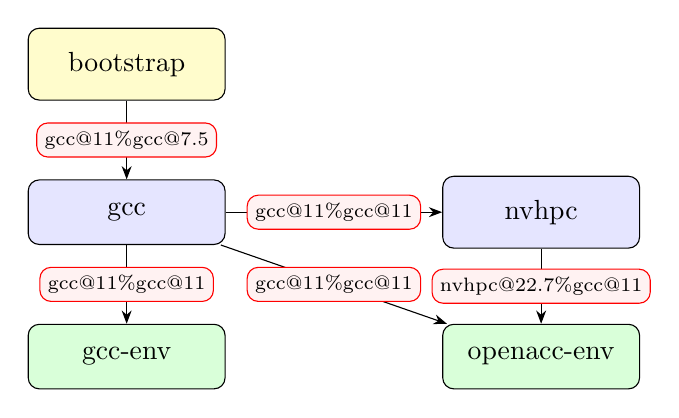
\begin{tikzpicture}[node distance=1cm and 2.75cm,
            nodes={draw, rectangle, rounded corners, minimum height=0.5cm, minimum width=2.5cm, fill=blue!10, inner sep=0.3cm},
            arrows={-Stealth}]
    % Nodes
    \node[fill=yellow!20] (bootstrap) {bootstrap};
    \node[below=of bootstrap] (gcc) {gcc};
    \node[right=of gcc] (nvhpc) {nvhpc};
    \node[fill=green!15, below=of gcc] (gcc-env) {gcc-env};
    \node[fill=green!15, right=of gcc-env] (openacc-env) {openacc-env};

    % Edges
    \draw (bootstrap)
        edge node[midway, fill=white,rectangle,fill=red!5, draw=red, inner sep=0.1cm, minimum height=0.3cm, minimum width=1 cm]
        {\scriptsize gcc@11\%gcc@7.5}
        (gcc);
    \draw (gcc) 
        edge node[midway, fill=white,rectangle,fill=red!5, draw=red, inner sep=0.1cm, minimum height=0.3cm, minimum width=1 cm]
        {\scriptsize gcc@11\%gcc@11}
        (nvhpc);
    \draw (gcc) 
        edge node[midway, fill=white,rectangle,fill=red!5, draw=red, inner sep=0.1cm, minimum height=0.3cm, minimum width=1 cm]
        {\scriptsize gcc@11\%gcc@11}
        (gcc-env);
    \draw (gcc) 
        edge node[midway, fill=white,rectangle,fill=red!5, draw=red, inner sep=0.1cm, minimum height=0.3cm, minimum width=1 cm]
        {\scriptsize gcc@11\%gcc@11}
        (openacc-env);
    \draw (nvhpc) 
        edge node[midway, fill=white,rectangle,fill=red!5, draw=red, inner sep=0.1cm, minimum height=0.3cm, minimum width=1 cm]
        {\scriptsize nvhpc@22.7\%gcc@11}
        (openacc-env);
\end{tikzpicture}

    \end{center}
\end{frame}
%-------------------------------------------

%-------------------------------------------
\begin{frame}[fragile]{Optimising Build Times}
    \begin{center}
        \begin{tikzpicture}[scale=1]
    \begin{axis} [
        ymin = 0, ymax=3000,
        ybar, bar width = 18pt,
        %symbolic x coords={1,2,3,4},
        grid=major,
        xtick = {1,2,3,4},
        xticklabels = {scratch, memory, cache, partial},
        xticklabel style={text height=1ex},
        ylabel={Build time (s)},
        nodes near coords,
        nodes near coords style={fill=white},
    ]
        \addplot[fill=orange!30] table[x=id, y=time-s] {./data/stack-build.tbl};
        \draw[line width=2pt, ->] (axis cs:2,2714) -- (axis cs:2,1866);
        \draw[line width=2pt, ->] (axis cs:3,1566) -- (axis cs:3,445);
        \draw[line width=2pt, ->] (axis cs:4,1566) -- (axis cs:4,787);
        \node[fill=white] () at (axis cs:2,2300) {\bfseries 1.7x};
        \node[fill=white] () at (axis cs:3,1000) {\bfseries 10.8x};
        \node[fill=white] () at (axis cs:4,1200) {\bfseries 3.2x};

        %\draw (s1_t.center) -- (s1_b.center);
    \end{axis}
\end{tikzpicture}


    \end{center}
\end{frame}
%-------------------------------------------


\cscschapter{Deploying spack-stacks}

%-------------------------------------------
\begin{frame}[fragile]{SquashFS}
    The images can be copied to a shared file system

    At CSCS they are compressed as SquashFS images:
    \begin{itemize}
        \item memory!
        \item performance! (don't bother with plots - just mention to save space)
        \item DevOps!
    \end{itemize}
\end{frame}
%-------------------------------------------

%-------------------------------------------
\begin{frame}[fragile]{CLI Utilities}
    Non-privileged users are able to mount SquashFS images at runtime using the \emph{squashfs-mount} CLI setuid utility that:
    \begin{enumerate}
    \item creates a new mount namespace
    \item mounts the SquashFS file through \emph{libmount}
    \item drops privileges and executes a given command.
    \end{enumerate}

    \begin{code}{mounting a squashfs image}
\lstinputlisting[style=talkyaml]{src/squashfs-mount.sh}
    \end{code}

    \begin{center}
        \textbf{The image is mounted in the new process -- processes (users) on the same node can mount different images.}
    \end{center}

    \vspace{10pt}

    Open Source on GitHub with RPMs for Cray EX.\\\url{https://github.com/eth-cscs/squashfs-mount}
\end{frame}
%-------------------------------------------

%-------------------------------------------
\begin{frame}[fragile]{SLURM}
    A Slurm plugin manages mounting environmnents on compute nodes.
    \begin{code}{Launch with explicit flags}
            \begin{lstlisting}[style=talkbash]
% srun --uenv-mount=/user-environment \
       --uenv-file=img.squashfs \
       -n2 -N2 osu_bw
            \end{lstlisting}
    \end{code}
    \begin{code}{Inherit the environment from the login node}
            \begin{lstlisting}[style=talkbash]
% squashfs-mount img.squashfs /user-environment bash
% srun -n2 -N2 osu_bw
            \end{lstlisting}
    \end{code}

    Also works intuitively for \emph{sbatch} -- user can set a default image that, and individual \emph{srun} in the script can use different environments.

    Open Source on GitHub with RPMs for Cray EX.\\\url{https://github.com/eth-cscs/slurm-uenv-mount/}
\end{frame}
%-------------------------------------------

%-------------------------------------------
\begin{frame}[fragile]{CI/CD}
    \begin{center}
    CI/CD pipelines \emph{from recipe to deployed SquashFS image} is a work in progress.
    \end{center}

    \vspace{10pt}

    Recipes are stored in a GitHub repository -- Pull requests and merges trigger a pipeline:
    \begin{enumerate}
        \item \emph{\sc Build Stage}: launch a Slurm job on the target cluster+architecture that uses stackinator to configure then build the image.
        \item push the generated image to a JFrog artifactory
        \item \emph{\sc Test Stage}: pull the image and run a Slurm job that executes ReFrame tests.
        \item post status to GitHub
        \item \emph{\sc Deploy Stage}: promote artifact to deployment artifactory (manual).
    \end{enumerate}
\end{frame}
%-------------------------------------------

\cscschapter{Results}

%-------------------------------------------
\begin{frame}[fragile]{OSU}
    We run OSU benchmarks compiled using CPE and Spack Stacks to understand the effect of packaging cray-mpich outside CPE.
\begin{center}
    \begin{tabular}{l |c  c }
                      & CPE   & Spack Stack \\
          \hline
        osu-benchmark & 5.9   & 5.9       \\
        cray-mpich    & 8.1.21& 8.1.24    \\
        gcc           & 11.2  & 11.3      \\
        cuda          & 11.6  & 11.8      \\
    \end{tabular}
\end{center}

    The benchmarks are run on \emph{Clariden}, a vCluster with \emph{64-core EPYC CPU} and  \emph{4 A100-80 GPUs} -- similar to Perlmutter.

\end{frame}
%-------------------------------------------

%-------------------------------------------
\begin{frame}[fragile]{OSU - P2P Bandwidth}
    \begin{center}
            \begin{tikzpicture}[scale=1]
        \begin{loglogaxis} [
            height=7cm, width=11cm,
            xmin = 1, xmax = 4194304,
            ymax = 40000, ymin=0.1,
            ytick={0.1,1,10,100,1000,10000},
            yticklabels={0.1,1,10,100,1000,10000},
            xtick={1,2,4,8,16,32,64,128,256,512,1024,2048,4096,8192, 16384,  32768,  65536,  131072, 262144, 524288, 1048576, 2097152, 4194304},
            xticklabels={1,2,4,8,16,32,64,128,256,512,1k,2k,4k,8k,16k,32k,64k,128k,256k,512k,1M,2M,4M},
            x tick label style={rotate=60,anchor=east},
            axis line style=very thick,
            ylabel=Bandwidth (MB/s),
            xlabel=Message Size,
            legend style = {at={(0.95,0.05)}, anchor=south east},
            grid=major
        ]
            \addplot[color=green!40!black,mark=square*,mark options={fill=white}, very thick]
                table[x=bytes, y=cpe-gpu-bw] {./data/osu/p2p.tbl};
            \addlegendentry{cpe/gpu}
            \addplot[color=orange!90!black,mark=*,mark options={fill=white}, very thick]
                table[x=bytes, y=sq-gpu-bw] {./data/osu/p2p.tbl};
            \addlegendentry{uenv/gpu}

            \addplot[color=blue!40!white,mark=square*,mark options={fill=white}, very thick]
                table[x=bytes, y=cpe-cpu-bw] {./data/osu/p2p.tbl};
            \addlegendentry{cpe/cpu}
            \addplot[color=yellow!70!black,mark=*,mark options={fill=white}, very thick]
                table[x=bytes, y=sq-cpu-bw] {./data/osu/p2p.tbl};
            \addlegendentry{uenv/cpu}

        \end{loglogaxis}
    \end{tikzpicture}

    \end{center}
\end{frame}
%-------------------------------------------

%-------------------------------------------
\begin{frame}[fragile]{OSU - P2P Latency}
    \begin{center}
        \input{images/osu-p2p-lat-slides.tex}
    \end{center}
\end{frame}
%-------------------------------------------

%-------------------------------------------
\begin{frame}[fragile]{GROMACS}
    A GROMACSD strong scaling benchmarks: a 1.4-million atom system (a pair of hEGFR Dimers of 1IVO and 1NQL) from the HECBioSim benchmarks suite.
\begin{center}
    \begin{tabular}{|l |c  c| }
        \cline{2-3}
\multicolumn{1}{c|}{} & CPE   & Spack Stack \\
        \hline
        gromacs       & 2021.5   & 2021.5   \\
        fftw          & 3.3.10   & 3.3.10   \\
        openblas      & 0.3.21   & 0.3.21   \\
        cray-mpich    & 8.1.21   & 8.1.24   \\
        gcc           & 11.2     & 11.3     \\
          \hline
    \end{tabular}
\end{center}

    Run on \emph{Clariden}, a vCluster with \emph{64-core EPYC CPU} and  \emph{4 Mi250x GPUs} -- identical to LUMI/Frontier/Setonix.
\end{frame}
%-------------------------------------------

%-------------------------------------------
\begin{frame}[fragile]{GROMACS - Strong Scaling}
    A difference of maximum $\pm$1.5\% between the CPE and the Spack-stack.
    \begin{center}
        \input{images/gromacs-slides.tex}
    \end{center}
\end{frame}
%-------------------------------------------

\cscschapter{Wrapping up}

\cscschapter{Thank you -- any questions?}



\end{document}
